\documentclass[aspectratio=169]{beamer}
\usepackage{fontspec}
\usefonttheme{professionalfonts}
\usepackage{amsmath,amssymb,amsthm}
\usepackage{arydshln,mathtools}
\usepackage{bm}
\usepackage{color}
\definecolor{theme}{RGB}{0,73,114}
\usepackage{multicol}
%\usepackage[caption=false]{subfig}
\usepackage{subcaption}
\usepackage{tikz-cd}


\usepackage{comment}

\usepackage{graphicx}
\usepackage{diffcoeff}
\usepackage{dsfont}
\usepackage{mathrsfs}
\usepackage[most]{tcolorbox}

\usepackage{xspace}
\usepackage{appendixnumberbeamer}


\usepackage{media9}
\usepackage[backend=bibtex, style=verbose]{biblatex}

\bibliography{biblio_PH}
%\renewcommand\bibfont{\scriptsize}

\addtobeamertemplate{footnote}{\vspace{-6pt}\advance\hsize-0.5cm}{\vspace{6pt}}
\makeatletter
% Alternative A: footnote rule
\renewcommand*{\footnoterule}{\kern -3pt \hrule \@width 2in \kern 8.6pt}
% Alternative B: no footnote rule
% \renewcommand*{\footnoterule}{\kern 6pt}
\makeatother


\makeatletter
\g@addto@macro\normalsize{%
	\setlength\abovedisplayskip{5pt}
	\setlength\belowdisplayskip{5pt}
	\setlength\abovedisplayshortskip{5pt}
	\setlength\belowdisplayshortskip{5pt}
}
\makeatother

\graphicspath{{./imagesPH/}}



% Math macros
\DeclareMathOperator*{\grad}{grad}
\DeclareMathOperator*{\Grad}{Grad}
\DeclareMathOperator*{\Div}{Div}
\renewcommand{\div}{\operatorname{div}}
\DeclareMathOperator*{\Hess}{Hess}
\DeclareMathOperator*{\curl}{curl}


\DeclareMathOperator{\tr}{tr}

\DeclareMathOperator{\Dom}{Dom}
\DeclareMathOperator*{\esssup}{ess\,sup}

\newcommand{\bbR}{\mathbb{R}}
\newcommand{\bbI}{\mathbb{I}}
\newcommand{\bbC}{\mathbb{C}}
\newcommand{\bbF}{\mathbb{F}}
\newcommand{\bbA}{\mathbb{A}}
\newcommand{\bbB}{\mathbb{B}}
\newcommand{\bbS}{\mathbb{S}}


\newcommand{\inpr}[3][]{\ensuremath{( #2, \, #3 )_{#1}}}
\newcommand{\dualpr}[3][]{\ensuremath{\langle #2 \, \vert #3 \rangle_{#1}}}

\newcommand{\bilprod}[2]{\langle \langle \, #1, #2 \, \rangle \rangle}
\newcommand*{\dual}[1]{\ensuremath{\widehat{#1}}}


\DeclareMathOperator*{\argmax}{arg\,max}
\DeclareMathOperator*{\argmin}{arg\,min}

\newtheorem{proposition}{Proposition}
\newtheorem{remark}{Remark}
\newtheorem{hypothesis}{Hypothesis}
\newtheorem{assumption}{Assumption}
\newtheorem{conjecture}{Conjecture}


\def\onedot{$\mathsurround0pt\ldotp$}
\def\cddot{% two dots stacked vertically
	\mathbin{\vcenter{\baselineskip.67ex
			\hbox{\onedot}\hbox{\onedot}}%
}}


\setbeamertemplate{blocks}[rounded][shadow]

\setbeamercolor{block body alerted}{bg=alerted text.fg!10}
\setbeamercolor{block title alerted}{bg=alerted text.fg!20}
\setbeamercolor{block body}{bg=structure!10}
\setbeamercolor{block title}{bg=structure!20}
\setbeamercolor{block body example}{bg=green!10}
\setbeamercolor{block title example}{bg=green!20}

% Remove navigation bar
\setbeamertemplate{navigation symbols}{}

\addtobeamertemplate{navigation symbols}{}{%
	\usebeamerfont{footline}%
	\usebeamercolor[fg]{footline}%
	\hspace{1em}%
	\insertframenumber/\inserttotalframenumber
}


\makeatletter \renewcommand\d[1]{\ensuremath{%
		\;\mathrm{d}#1\@ifnextchar\d{\!}{}}}
\makeatother


%% At begin of each section: show current section and all subsections in the section if any
%% At begin of each subsection except first: show only the current section/subsection
\newif\iftocsub
\tocsubtrue
\AtBeginSection[] {
	\begin{frame}[noframenumbering]{Outline}
		\tableofcontents[sectionstyle=show/shaded, subsectionstyle=show/show/hide]
	\end{frame}
	\tocsubfalse
}
\AtBeginSubsection[] {
	\iftocsub
	\begin{frame}[noframenumbering]{Outline}
		\tableofcontents[currentsubsection, sectionstyle=show/shaded, subsectionstyle=show/shaded/hide]
	\end{frame}
	\fi
	\tocsubtrue
}

\newcommand{\beginbackup}{
	\newcounter{framenumbervorappendix}
	\setcounter{framenumbervorappendix}{\value{framenumber}}
}
\newcommand{\backupend}{
	\addtocounter{framenumbervorappendix}{-\value{framenumber}}
	\addtocounter{framenumber}{\value{framenumbervorappendix}} 
}


\begin{document}
	
	
	\begin{frame}[plain]
		
		%%%%%%%% Title slide details %%%%%%%%%%%%%%


% Background Image
\newcommand{\myBackground}
{
    
\includegraphics[height=1.02\paperheight,page=9]{beamerthemeutresources}
}

% Title
\newcommand{\myTitle}
{
Improving multiphysics simulation through port-Hamiltonian system theory
}

% Subtitle
\newcommand{\mySubTitle}
{
}

% Author
\newcommand{\myAuthor}   
{
    Andrea Brugnoli
}

% Affiliation
\newcommand{\myAffiliate}
{
  
}

% Presentation Date
\newcommand{\myDate}   
{
    28 June 2022
}

% Logo
\newcommand{\myLogo}   
{
    
\includegraphics[width=3cm]{Logo.png}
}
%%%%%%%%%%%%%%%%%%%%%%%%%%%%%%%%%%%%


%%%%%%%%%% Title slide code %%%%%%%%%%%
\begin{tikzpicture}[remember picture,overlay]

% Background color

\fill[white] (current page.south west) rectangle (current page.north east);
% Background image
\node[above right,inner sep=0pt] at (current page.south west)
    {
        \myBackground
    };
    
% Title & Subtitle
\node
[
    above=0.5cm,
    align=center,
    draw=black!50,
    % rounded corners,
    double,
    double distance=0.1cm,
    double=blue!10,
    fill=theme!10,
    inner xsep=15pt,
    inner ysep=10pt, 
    minimum width=0.8\textwidth,
    text width=0.8\textwidth
] (title) at (current page.center)
{
    \LARGE \myTitle  \\[5pt]
    \small \mySubTitle
};

% Author 
\node[ below=0.5cm] (author) at (title.south){\myAuthor};

% Author 
\node[ below=0.25cm ](affiliate) at (author.south){\small \myAffiliate};

% Date
\node[below=0.25] (date) at (affiliate.south){\large \myDate};

% Logo
\node
[
    below =0.25cm
] at (date.south)
{
    \myLogo
};

\end{tikzpicture}
		
	\end{frame}
	
	
	\begin{frame}{Outline}
		
		\tableofcontents
		
	\end{frame}

\section{Multiphysics problems}


\begin{frame}{Challenges in muliphysics problems}
	
	Multiphysics problems are commonly found in industrial applications.
	\begin{figure}[t]
		\begin{subfigure}[t]{0.34\textwidth}
			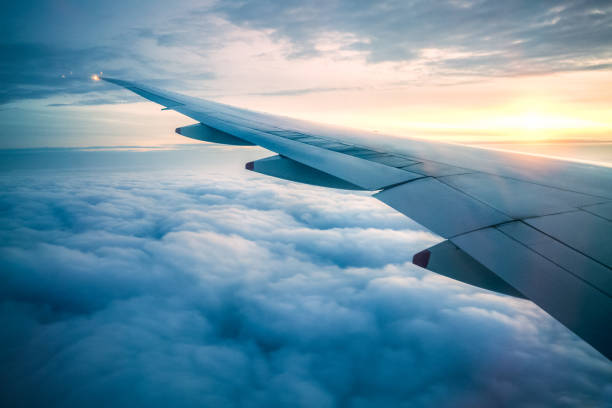
\includegraphics[width=\columnwidth]{wing.jpg}\\
			\centering{Aeroelasticity}%
		\end{subfigure}\hfill
		\begin{subfigure}[t]{0.3\textwidth}
			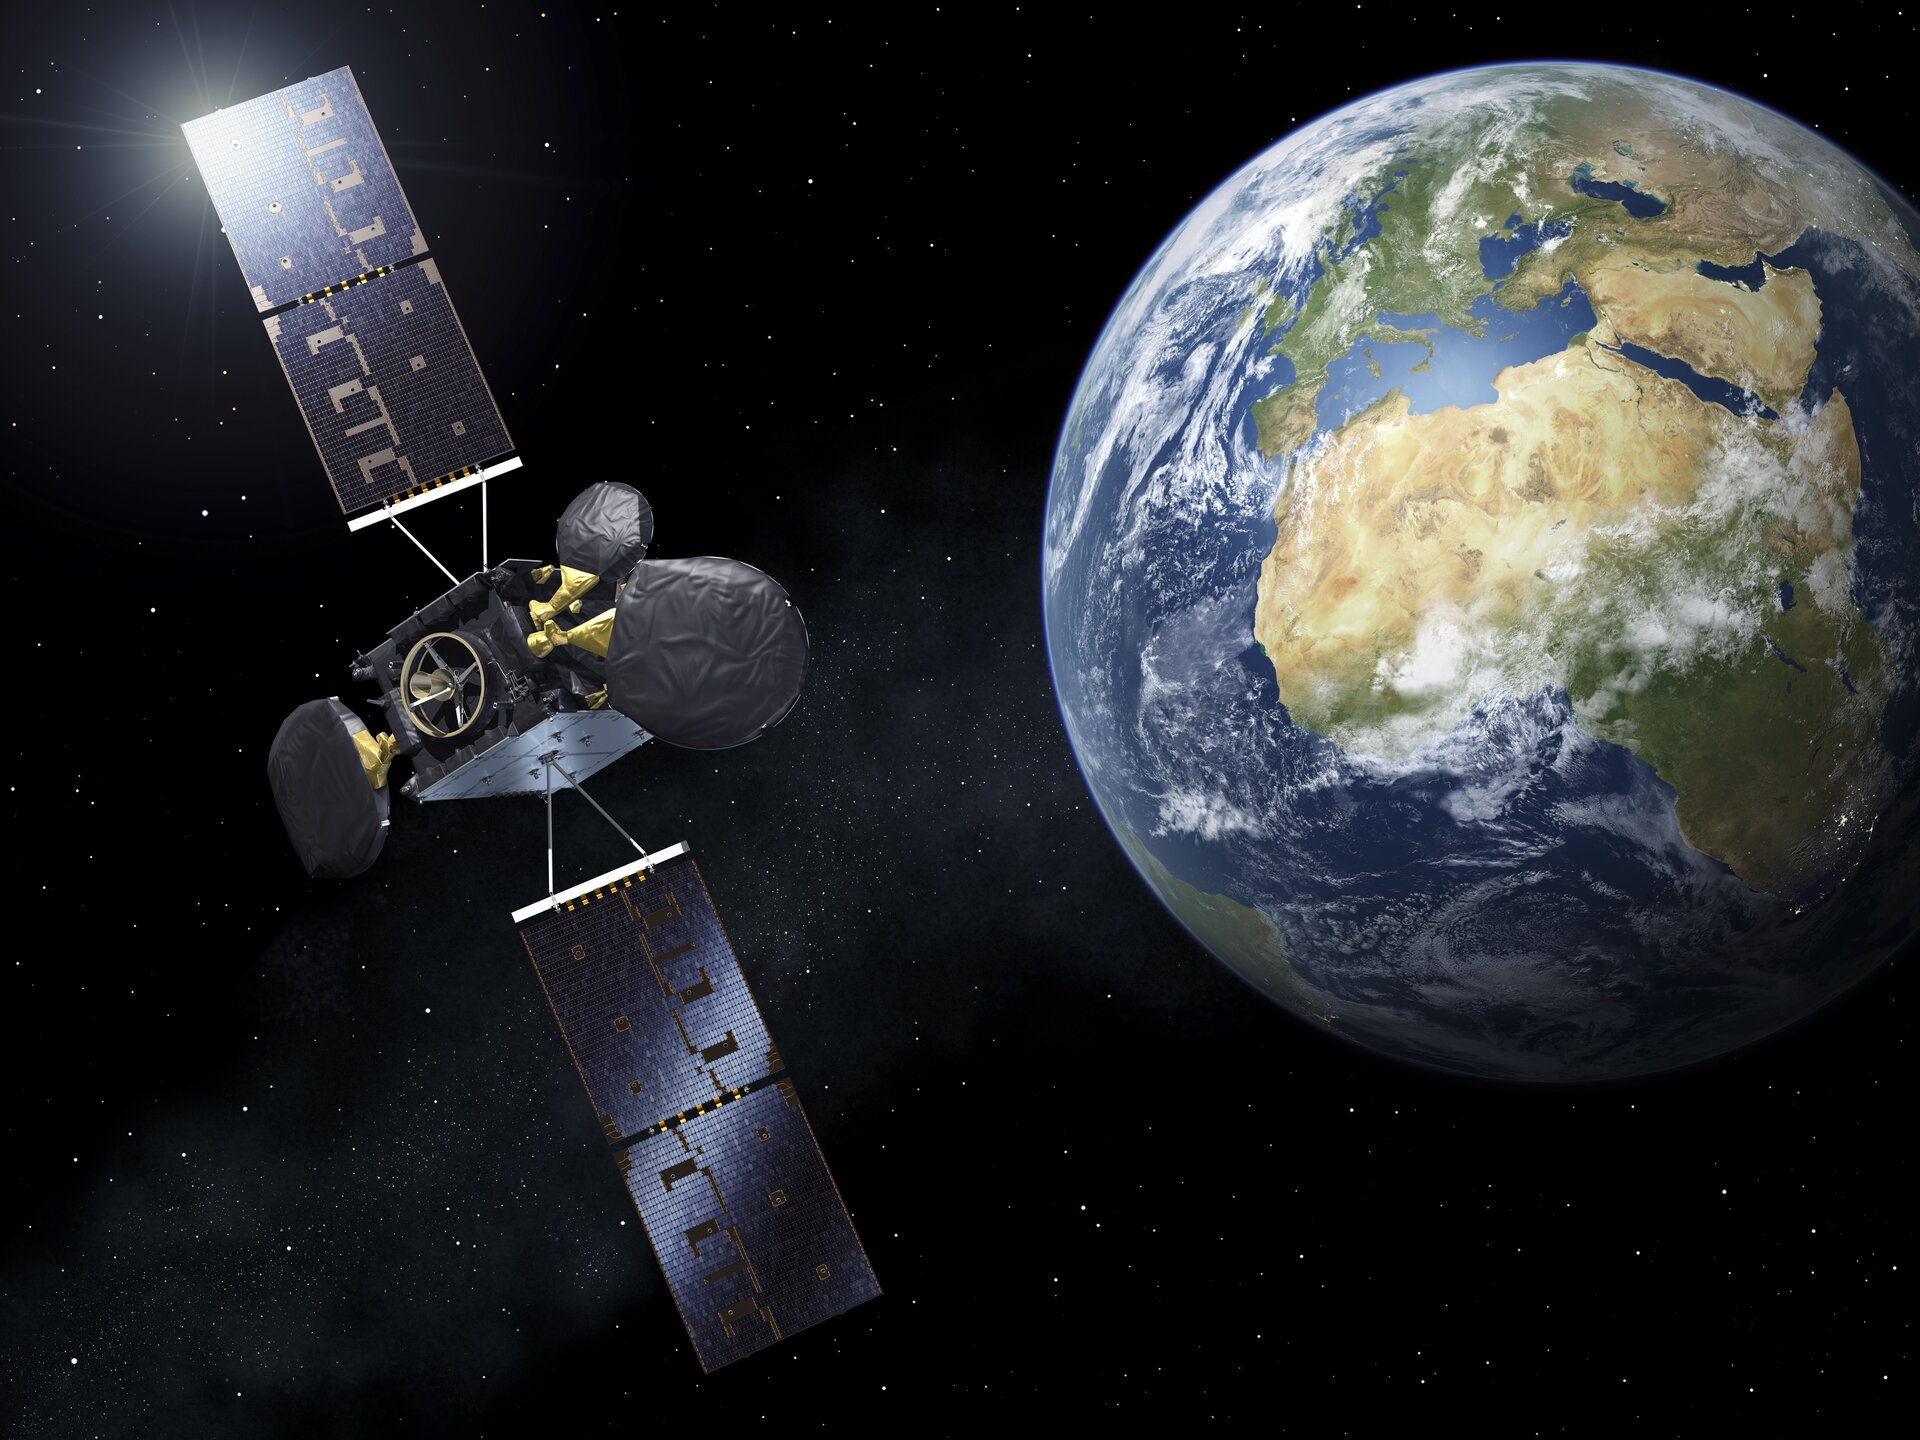
\includegraphics[width=\columnwidth]{esa_satellite.jpg}\\
			\centering{Thermoelasticity} 
		\end{subfigure}\hfill
		\begin{subfigure}[t]{0.26\textwidth}
			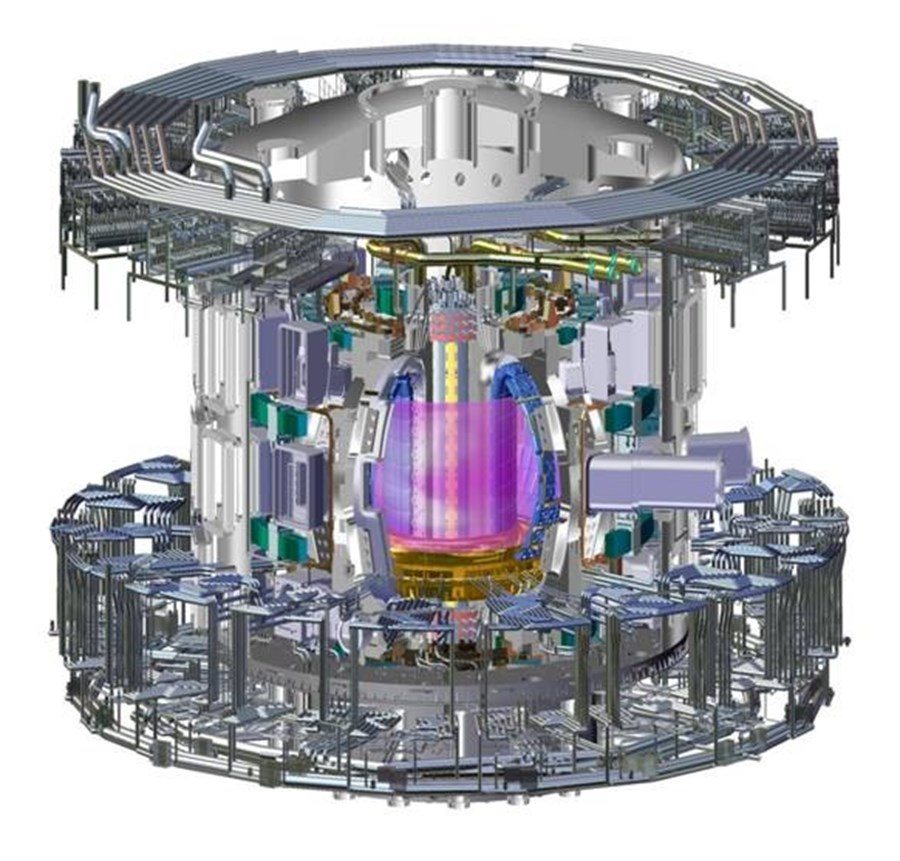
\includegraphics[width=\columnwidth]{tcws.jpg}\\
			\centering{Magnetohydrodynamics}
		\end{subfigure}
	\end{figure}
	Challenges:
	\begin{itemize}
		\item Coupling between different models.​
		\item Huge computational cost due to the large size of the models.​
		\item Multidisciplinary optimization for dynamical systems.​
	\end{itemize}
	
\end{frame}


\begin{frame}{Typical workflow in industry}
	
	\begin{itemize}
		\item \textbf{Specific modelling} and numerical methods for each physical domain. 
			\begin{itemize}
			\item[$-$] The \textbf{open character} of systems is \textbf{not considered}.
			\item[$-$] Numerical methods do not preserve the structure required to interconnect systems.
		\end{itemize}
		\item Model reduction via statistical methods.
	\begin{itemize}
		\item[$-$] The \textbf{physical structure is lost} and first principles are violated.
		\item[$-$] This methodology \textbf{does not generalize} to different problems.
	\end{itemize}
\vspace{.3cm}
	\begin{figure}[t]
		\centering
		\begin{subfigure}[t]{0.4\textwidth}
			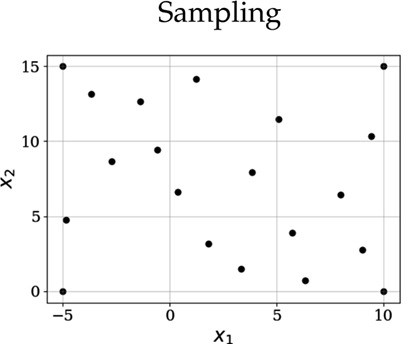
\includegraphics[width=.8\columnwidth]{sampling.jpg}
		\end{subfigure}\hspace{1cm}
		\begin{subfigure}[t]{0.4\textwidth}
			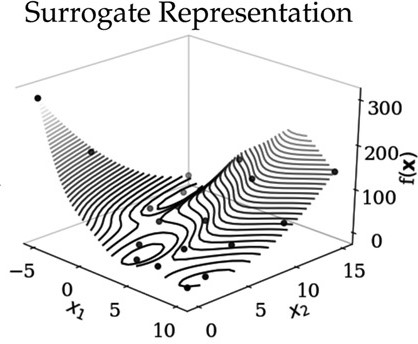
\includegraphics[width=.8\columnwidth]{surrogate_model.jpg}
		\end{subfigure}
	\end{figure}
	\end{itemize}
\end{frame}

\begin{frame}{Example: convection dominated transport}
	Convection dominated transport of a passive scalar field in a Stokes flow\footcite{volker2017review}
	\begin{equation*}
		\begin{aligned}
			\nu \Delta \bm{u} + \nabla p &=0, \\
			\nabla \cdot \bm{u} &=0, \\
			-\varepsilon \Delta \theta + \bm{u} \cdot \nabla \theta &=0.
		\end{aligned} \qquad \qquad 
	\begin{aligned}
		\bm{u} &: \text{Velocity}, \\
		p &: \text{Pressure}, \\
		\theta &: \text{Temperature}.
	\end{aligned}
	\end{equation*}
	\begin{figure}
		\centering
		\includegraphics[width=.7\textwidth]{channel_convection_T.eps}
		\caption*{Geometry and boundary conditions}
	\end{figure}
\end{frame}

\begin{frame}{When multiphysics goes wrong}
	Exact solution for the temperature $\theta_{\mathrm{ex}}= 1$.
	\begin{itemize}
		\item $(\bm{u}_h, p_h)$ represented using the Taylor-Hood element $\mathbb{P}_2/\mathbb{P}_1$;
		\item $\theta_h$ obtained via Voronoi finite volume method.
	\end{itemize}
The Taylor-Hood element does not lead to divergence free velocity $||\nabla \cdot \bm{u}_h||_{L^2(\Omega)} \neq 0$.
\begin{figure}[t]
	\begin{subfigure}[t]{0.32\textwidth}
		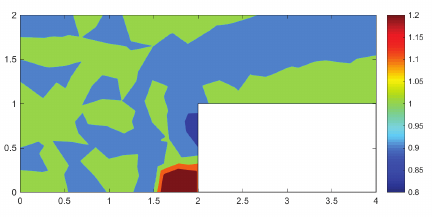
\includegraphics[width=\columnwidth]{Concentration_ref1.png}\\
		\centering{Refinement 1}%
	\end{subfigure}\hfill
	\begin{subfigure}[t]{0.32\textwidth}
		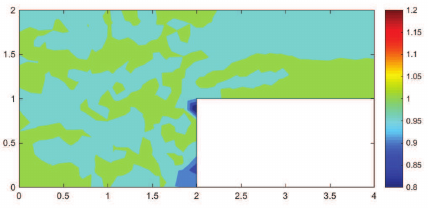
\includegraphics[width=\columnwidth]{Concentration_ref2.png}\\
		\centering{Refinement 2} 
	\end{subfigure}\hfill
	\begin{subfigure}[t]{0.32\textwidth}
		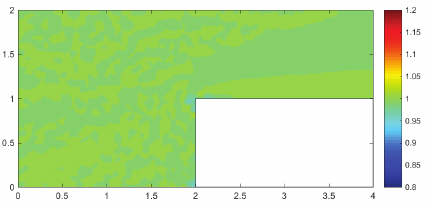
\includegraphics[width=\columnwidth]{Concentration_ref3.png}\\
		\centering{Refinement 3}
	\end{subfigure}
\caption{Discrete temperature field $\theta_h$ obtained }
\end{figure}

\end{frame}

\section{Port-Hamiltonian systems as a unified language for multiphysics}

\begin{frame}{A unified language for multiphysics in engineering}
	The port-Hamiltonian (pH) paradigm provides a language to understand multiphysics:
	\vspace{.3cm}
	\begin{columns}
		\begin{column}{.65\textwidth}
			\begin{itemize}
				\item \textbf{Physics} is at the core: port-Hamiltonian systems are \textbf{passive} with respect to the \textbf{energy storage function}.
				\item The \textbf{topological} and \textbf{metrical} structure of the equation is clearly separated (mimetic discretization).
				\item PH systems are \textbf{closed under interconnection}. 
			\end{itemize}
		\end{column}
		\begin{column}{.35\textwidth}
			\centering
			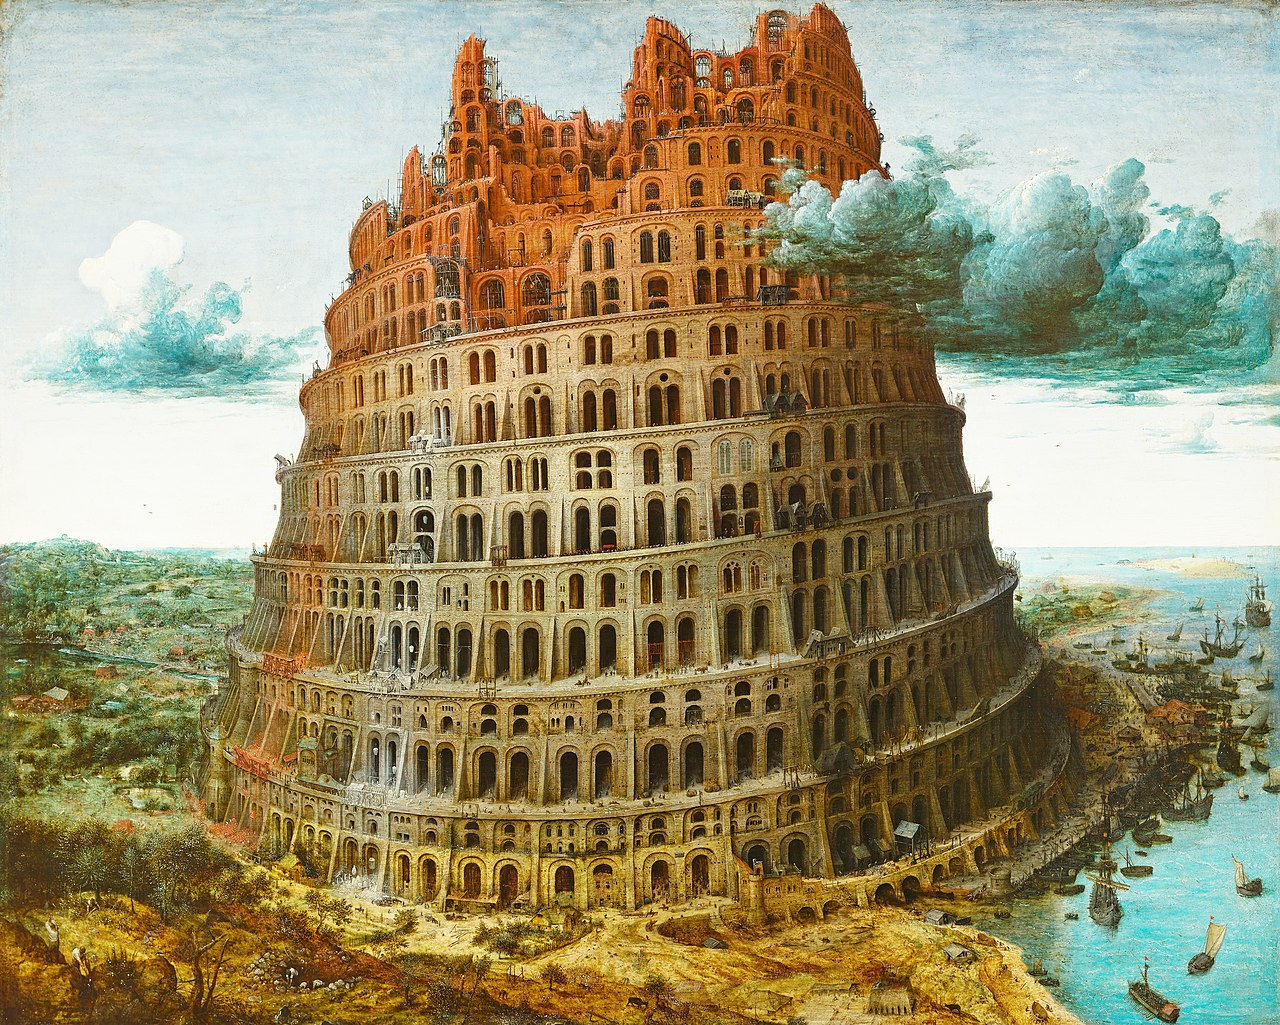
\includegraphics[width=.9\columnwidth]{babel_tower.jpeg}
		\end{column}
	\end{columns}
\begin{block}{A quest for duality}
	The concept of \textbf{interconnection} and the \textbf{port} behavior of pH systems is mathematically formalized as \textbf{duality pairing}. How exactly is that defined?
\end{block}


\end{frame}

\begin{frame}{Finite dimensional pH systems}

\begin{alertblock}{A theory still under developement}
	There is \textbf{not a unique definition} of pH systems, even in finite dimension.
\end{alertblock}

\begin{definition}[Finite dimensional pH system]
	
	The time-invariant dynamical system
	\begin{equation*}
		\begin{aligned}
			\dot{\mathbf{x}} &= \left( \mathbf{J} - \mathbf{R} \right) \nabla_{\mathbf{x}} H + \mathbf{B}\mathbf{u}, \\
			\mathbf{y} &= \mathbf{B}^\top ~ \nabla_{\mathbf{x}} H,
		\end{aligned}
	\end{equation*}
	where $\mathbf{x}$ is the state, $\mathbf{u}$ the control input, $\mathbf{y}$ the collocated output and
	\begin{itemize}
		\item $H(\mathbf{x}) : \mathbb{R}^n \rightarrow \mathbb{R}$, the Hamiltonian, is bounded from below.
		\item $\mathbf{J}=-\mathbf{J}^\top $ the interconnection operator.
		\item $\mathbf{R}=\mathbf{R}^\top \in \bbR^{n \times n}, \; \mathbf{R} \ge 0$ the resistive operator.
		\item $\mathbf{B} \in \bbR^{n \times m}$ the control operator.
	\end{itemize}
	is a pH system.
\end{definition}

\end{frame}


\begin{frame}{The geometric structure of pH systems\footcite{courant1990}}
	\begin{definition}[Dirac structure]
		Given a vector space ${F}$ and its dual ${E}=F'$ with respect to the duality product $\dualpr{\cdot}{\cdot} : {E} \times {F} \rightarrow \mathbb{R}$, consider the symmetric bilinear form:
		$$
		\bilprod{({f}_1, {e}_1)}{({f}_2, {e}_2)} := {\dualpr{{e}_1}{{f}_2}} + {\dualpr{{e}_2}{{f}_1}}, \qquad ({f}_i, {e}_i) \in {B} = {F} \times {E}, \; i = 1, 2.
		$$
		A Dirac structure is a linear subspace $\mathcal{D} \subset {B}$ which equals its orthogonal companion with respect to $\left\langle \left\langle \cdot, \cdot \right\rangle \right\rangle$, {\it i.e.} $\mathcal{D} =\mathcal{D}^{[\perp]}$, where:
		$$
		\mathcal{D}^{[\perp]} := \left\{ ({f}, {e}) \in {B} ~ \mid ~ \bilprod{({f}, {e})}{(\widehat{{f}}, \widehat{{e}})} = 0, ~ \forall ~ (\widehat{{f}}, \widehat{{e}}) \in \mathcal{D} \right\}.
		$$
	\end{definition}
	\begin{theorem}[Finite dimensional Dirac structure]
		A subspace $\mathcal{D} \subset F \times E$ where $F$ is a finite-dimensional vector space ${F}$ and ${E}=F'$ its dual is a Dirac structure if and only if $\dualpr{\mathbf{e}}{\mathbf{f}}=0$ and $\mathrm{dim}\, D = \mathrm{dim}\, F$.
	\end{theorem}
\end{frame}

\begin{frame}{Dirac structure and pH systems}
	
	From classical matrix factorization $\exists \, \mathbf{G} \in \bbR^{k \times n}$ and $\mathbf{K} = \mathbf{K}^\top \in \bbR^{k \times k}, \; \mathbf{K} \ge 0$ such that $\mathbf{R} = \mathbf{G}^\top ~ \mathbf{K} \mathbf{G}$. \\
	\vspace{.2cm}
	
	\begin{tcolorbox}[nobeforeafter, colframe=theme,title=Dirac structure representation]%%
			Considering the following \textbf{port behavior}:
		\begin{itemize}
			\item
			the \textbf{storage ports} $(\mathbf{f}_{{x}}, \mathbf{e}_{{x}}) := \left(-\dot{\mathbf{x}}, \nabla_{\mathbf{x}} H \right) \in \mathbb{R}^n \times \mathbb{R}^n$;
			\item
			the \textbf{resistive ports} $(\mathbf{f}_{r}, \mathbf{e}_{r}) \in \mathbb{R}^k \times \mathbb{R}^k$;
			\item
			the \textbf{interconnection ports} $(\mathbf{f}_{{u}}, \mathbf{e}_{{u}}) := (\mathbf{y}, \mathbf{u} ) \in \mathbb{R}^m \times \mathbb{R}^m$.
		\end{itemize}
		Given this port behavior, the pH system rewrites
		\begin{equation*}
			\begin{pmatrix}
				-\dot{\mathbf{x}} \\
				\mathbf{f}_{r} \\
				\mathbf{f}_{u}
			\end{pmatrix}
			=
			\underbrace{\begin{bmatrix}
					-\mathbf{J}	& \mathbf{G}^\top	& -\mathbf{B} \\
					\mathbf{G} 	& \mathbf{0}		& \mathbf{0} \\
					\mathbf{B}^\top	& \mathbf{0}	& \mathbf{0} \\
			\end{bmatrix}}_{\mathbf{J}_e}
			\begin{pmatrix}
				\nabla_{\mathbf{x}} H\\
				\mathbf{e}_{r}\\
				\mathbf{e}_{u}
			\end{pmatrix}, \qquad \mathbf{e}_{r} = \mathbf{K} \mathbf{f}_{r}.
		\end{equation*}
		
		Since $\mathbf{J}_e$ is skewsymmetric its graph $\{(\mathbf{f}, \mathbf{e}) \in F \, |\, \mathbf{f}=\mathbf{J}_e \mathbf{e}\}$ is a Dirac structure.
	\end{tcolorbox} 
	
\end{frame}


\subsection{Functional analytic structure}

\begin{frame}{A simple definition\footcite{reis2021pH}}
	\begin{definition}[Port-Hamiltonian system]
		Let $X_\mathcal{S}, \; X_\mathcal{R}, \; {X}_{\mathcal{P}}$ be Banach spaces. A port-Hamiltonian system is a triple $(\mathcal{D}, H, \mathcal{R})$:
		\begin{itemize}
			\item $\mathcal{D} \subset (X_\mathcal{S}, \; X_\mathcal{R}, \; X_\mathcal{P}) \times (X^{'}_\mathcal{S}, \; X^{'}_\mathcal{R}, \; X^{'}_\mathcal{P})$ is a Dirac structure.
			\item ${H} : U \rightarrow \bbR$ (with $U \subset X_\mathcal{S}$ open) is a Hamiltonian.
			\item $\mathcal{R}\subset X_\mathcal{R} \times X_{\mathcal{R}}^{'}$ is a resistive relation.
		\end{itemize}
		The behavior of the pH system on an interval $\mathbb{I} \subset \bbR$ consists of all $(x, f_{\mathcal{R}}, f_{\mathcal{P}} , e_{\mathcal{R}}, e_{\mathcal{P}})$
		\begin{itemize}
			\item 	$x \in W^{1,2}_{\text{loc}}(\mathbb{I}, X_{\mathcal{S}})$, and $x(t) \in U, \; \forall t \in \bbI$, 
			\item $(f_\mathcal{R}, e_\mathcal{R}) \in L^2_{\text{loc}}(\bbI; X_{\mathcal{R}} \times X^{'}_{\mathcal{R}})$ and $(f_\mathcal{P}, e_\mathcal{P}) \in L^2_{\text{loc}}(\bbI; X_{\mathcal{P}} \times X^{'}_{\mathcal{P}})$
		\end{itemize}
		that fulfill the differential inclusion
		\begin{equation*}
			(-\partial_t x,\, f_{\mathcal{R}},\, f_{\mathcal{P}},\, D_x {H},\, e_{\mathcal{R}},\, e_{\mathcal{P}}) \in \mathcal{D}, \qquad (f_\mathcal{R}, e_\mathcal{R}) \in \mathcal{R}, \qquad \text{for almost all } t \in \bbI.
		\end{equation*}
	\end{definition}
\end{frame}

\begin{frame}
	\begin{block}{Dirac structure}
			Let $X$ be a Banach space. A subspace $\mathcal{D}\subset X \times X^{'}$ is called a Dirac structure, if $\forall \, f \in X, e \in X^{'}$, it holds
			\begin{equation*}
				(f, e) \in \mathcal{D} \iff \left( \dualpr{\widehat{e}}{f} + \dualpr{e}{\widehat{f}}=0, \quad \forall\, (\widehat{f}, \widehat{e}) \in \mathcal{D}\right).
			\end{equation*}
		\end{block}

		\begin{block}{Hamiltonian}
			Let $X$ be a Banach space and $U \subset X$ be open. A mapping ${H} : U \rightarrow \bbR$ is a Hamiltonian if it is locally Lipschitz continuous and G\^{a}teaux differentiable
		\end{block}
		
		\begin{block}{Resistive relation}
			Let $X$ be a Banach space.
			A relation $\mathcal{R} \subset X \times X^{'}$ is called resistive, if
			\begin{equation*}
				\dualpr{e}{f} \le 0, \qquad \forall\, (f,e) \in \mathcal{R}.
			\end{equation*}
		
		\end{block}

\end{frame}

\begin{frame}{Operators}
	If $J \in \mathcal{L}(X^{'}, X)$ is a skew-dual operator $\dualpr{w}{J v}= \dualpr{v}{-Jw}\; \forall\, v, w \in X^{'}$ then $\mathcal{D} = \{(J e, e) : e \in X^{'}\}$ is a Dirac structure\footcite{reis2022passivity}.\\
	\vspace{.2cm}
	If $K :X \rightarrow X^{'}$ is dissipative $\dualpr{K(x)}{x} \le 0,\; \forall \, x \in X$, then $\mathcal{R} = \{(K(f), f) : e \in X^{'}\}$ is a resistive relation.
	
	\begin{equation*}
		\begin{pmatrix}
			-\partial_t x \\
			f_\mathcal{R} \\
			f_\mathcal{P} \\
		\end{pmatrix} =
		J
		\begin{pmatrix}
			D_x\mathcal{H} \\
			e_\mathcal{R} \\
			e_\mathcal{P} \\
		\end{pmatrix}, \qquad e_{\mathcal{R}} = K(f_{\mathcal{R}}).
	\end{equation*}
\end{frame}


\begin{frame}{Example: the wave equation}
	Consider the Hamiltonian
	\begin{equation*}
		{H} = \inpr[L^2(\bbR^3)]{p}{\kappa p} + \inpr[L^2(\bbR^3; \bbR^3)]{\bm{v}}{\rho^{-1}\bm{v}}.
	\end{equation*}
	where $\kappa$ is the Bulk modulus and $\rho$ is the density. \\
	\vspace{.3cm}
	\begin{tcolorbox}[nobeforeafter, colframe=theme,title=The wave equation on $\bbR^3$ with distributed input]%%
	\begin{equation*}
		\begin{aligned}
			\diffp{}{t}
			\begin{pmatrix}
				p \\
				\bm{v} \\
			\end{pmatrix} &=-
			\begin{bmatrix}
				0 & \div \\
				\grad_w & 0
			\end{bmatrix}
			\begin{pmatrix}
				D_p{H} \\
				D_{\bm{v}}{H}\\
			\end{pmatrix} + \begin{bmatrix}
				\mathrm{Id} \\
				0
			\end{bmatrix} u, \qquad \grad{}_{w} \text{ is the weak gradient},\\
			y &= \begin{bmatrix}
				\mathrm{Id} & 0
			\end{bmatrix} \begin{pmatrix}
				D_p{H} \\
				D_{\bm{v}}{H}\\
			\end{pmatrix},
		\end{aligned}
	\end{equation*}
	\textbf{Spaces}: $X_{\mathcal{S}}= L^2(\bbR^3) \times H^{\div}(\bbR^3)^{'}, \; X_{\mathcal{R}} = \emptyset, \; X_{\mathcal{P}}= L^{2}(\bbR^3)$.
	\begin{equation*}
		J = \begin{bmatrix}
			0 & \div & - \mathrm{Id} \\
			\grad_w & 0 & 0 \\
			\mathrm{Id} & 0 & 0 
		\end{bmatrix}.
	\end{equation*}
	\end{tcolorbox} 
	


\end{frame}

\begin{frame}{Example: the Maxwell equations}
	Consider the Hamiltonian:
	\begin{equation*}
		{H} = \frac{1}{2} \inpr[L^2(\Omega; \bbR^3)]{\bm{D}}{\varepsilon^{-1}\bm{D}} + \frac{1}{2} \inpr[L^2(\Omega; \bbR^3)]{\bm{B}}{\mu^{-1}\bm{B}}.
	\end{equation*}
where  $\varepsilon$ is the electric permittivity and $\mu$ is the magnetic permeability.\\
\vspace{.3cm}
\begin{tcolorbox}[nobeforeafter, colframe=theme,title=The Maxwell equation on $\Omega \subset \bbR^3$ with conducting boundary condition]%%
	\begin{equation*}
		\diffp{}{t}\begin{pmatrix}
			\bm{D} \\ \bm{B} 
		\end{pmatrix} = 
		\begin{bmatrix}
			0 & \curl_w \\
			-\curl & 0 \\
		\end{bmatrix}
		\begin{pmatrix}
			D_{\bm{D}}{H} \\
			D_{\bm{B}}{H} \\
		\end{pmatrix},\qquad 
	\begin{aligned}
		\nabla \cdot \bm{D}= 0, \qquad	\nabla \cdot \bm{B}= 0, \\
			D_{\bm{D}}{H} \times \bm{n}|_{\partial\Omega}= \bm{E} \times \bm{n}|_{\partial\Omega}=0,
	\end{aligned}
	\end{equation*}
	where $\curl_w$ corresponds to a weak $\curl$ operator

	\textbf{Spaces}: $X_{\mathcal{S}}=H^{\curl}_0(\Omega| \div=0)^{'} \times L^2(\Omega; \bbR^3|\div=0), \; X_{\mathcal{R}} = \emptyset, \; X_{\mathcal{P}}= \emptyset$. 
	\begin{equation*}
		J = \begin{bmatrix}
			0 & -\curl_w \\
			\curl & 0 \\
		\end{bmatrix}.
	\end{equation*}
\end{tcolorbox} 

	
	
\end{frame}

\begin{frame}{And many more}
	The same framework applies to
	\begin{itemize}
		\item Linear and non-linear solid mechanics (beams, plates, shells, etc.).\\
		\item Fluid dynamics. \\
		\item Chemical reactions.
	\end{itemize}

\begin{tcolorbox}
However some aspects need further clarification:
\begin{itemize}
	\item how to describe generic boundary conditions?
	\item how to represent the duality in a discrete setting?
\end{itemize}
\end{tcolorbox}
\end{frame}





\subsection{The geometric formulation}


\begin{frame}{Geometric Dirac structure\footcite{vanderSchaft2002}}
	\begin{tcolorbox}[nobeforeafter, colframe=theme,title=Dirac structure for differential forms]%%
	On a Riemannian oriented manifold $\Omega$ consider
	\begin{itemize}
		\item the flows $(f^p_1, \, f^q_2, \, f_\partial^{n-p}) \in F = \Lambda^p(\Omega) \times \Lambda^q(\Omega) \times \Lambda^{n-p}(\partial\Omega)$,
		\item the efforts $(e_1^{n-p}, \, e_2^{n-q}, \, e_\partial^{n-q}) \in E = \Lambda^{n-p}(\Omega) \times \Lambda^{n-q}(\Omega) \times \Lambda^{n-q}(\partial\Omega)$,
	\end{itemize}
	with $p+q=n+1$ and $\Lambda^k(\Omega)$ is the space of smooth $k$-forms. \\
	The following subset $\mathcal{D} \subset F \times E$ defines a Dirac structure
	\begin{equation*}
		\begin{pmatrix}
			{f}^p_1 \\
			{f}^q_2
		\end{pmatrix} = 
		\begin{bmatrix}
				0 & (-1)^{pq+1} \d \\
				\d & 0 \\
		\end{bmatrix}
		\begin{pmatrix}
			{e}^{n-p}_1 \\
			{e}^{n-q}_2
		\end{pmatrix}, \qquad 
		\begin{pmatrix}
			{f}_\partial^{n-p} \\
			{e}_\partial^{n-q}
		\end{pmatrix} = 
		\begin{bmatrix}
			\tr & 0 \\
			0 &  (-1)^p\tr
		\end{bmatrix}
		\begin{pmatrix}
			{e}^{n-p}_1 \\
			{e}^{n-q}_2
		\end{pmatrix}.
	\end{equation*}
The key is that this subset verify the following power balance (Stokes formula)
\begin{equation*}\label{eq:bal_eq}
	\dualpr[\Omega]{e^{n-p}_1}{{f}^p_1} + \dualpr[\Omega]{{e}^{n-q}_2}{f^q_2} + \dualpr[\partial\Omega]{{e}_\partial^{n-q}}{{f}_\partial^{n-p}} = 0.
\end{equation*}
\end{tcolorbox} 

	
\end{frame}

\begin{frame}{Hyperbolic dynamical systems}
	Consider the following dynamical system with boundary input and observation
	\begin{equation*}
	\begin{aligned}
		\begin{pmatrix}
			\partial_t \alpha^p \\
			\partial_t \beta^q\\
		\end{pmatrix} &= 
		-\begin{bmatrix}
			0 & (-1)^{pq+1}\d \\
			\d & 0 \\
		\end{bmatrix}
		\begin{pmatrix}
			\delta_{\alpha} H^{n-p}\\
			\delta_{\beta} H^{n-q}\\
		\end{pmatrix}, \qquad (-1)^p\tr \delta_{\beta} H^{n-q} = u^{n-q}, \\
		y^{n-p} &= \tr \delta_{\alpha} H^{n-p}, 
	\end{aligned}	
	\end{equation*}
where the variational derivative is defined by
\begin{equation*}
	\begin{aligned}
		\left.\diff{}{\varepsilon}\right|_{\varepsilon = 0} H({\mu}^k + \varepsilon \delta {\mu}^k) = \dualpr[\Omega]{\delta_{\mu} H^{n-p}}{\delta {\mu}^k},
	\end{aligned}
\end{equation*}
Considering the following \textbf{port behavior}:
\begin{itemize}
	\item
	the \textbf{storage ports} $({f}_1^p,\, f_2^q,\, e_1^{n-p}, \, e_2^{n-q}) := (-\partial_t \alpha^p,\,  -\partial_t \beta^q, \,  \delta_{\alpha} H^{n-p}, \,  \delta_{\beta} H^{n-q})$;
	\item
	the \textbf{interconnection ports} $({f}_{\partial}^{n-p}, {e}_{\partial}^{n-q}) := ({y}^{n-p}, {u}^{n-q} )$.
\end{itemize}
Then the dynamical system defines a Dirac structure.

\end{frame}

\begin{frame}{The geometric wave and Maxwell equations}
	Assume $\Omega \subset \bbR^3$. \\
	Case $p=3, \; q=1$ Wave equation.
	\begin{equation*}
			\begin{aligned}
				\begin{pmatrix}
					\partial_t p^3 \\
					\partial_t \bm{v}^1\\
				\end{pmatrix} &= 
				-\begin{bmatrix}
					0 & \div \\
					\grad & 0 \\
				\end{bmatrix}
				\begin{pmatrix}
					\delta_{p} H^{0}\\
					\delta_{\bm{v}} H^{2}\\
				\end{pmatrix}, \qquad -\delta_{\bm{v}} H^{2} \cdot \bm{n}|_{\partial\Omega}  = u^{2}, \\
				y^{0} &= \delta_{p} H^{0}|_{\partial\Omega}.
			\end{aligned}	
	\end{equation*}
	\vspace{.5cm}\\
	Case $p=2, \;q=2$ Maxwell equation
	\begin{equation*}
		\begin{aligned}
			\begin{pmatrix}
				\partial_t \bm{D}^2 \\
				\partial_t \bm{B}^2\\
			\end{pmatrix} &= 
			\begin{bmatrix}
				0 & \curl \\
				-\curl & 0 \\
			\end{bmatrix}
			\begin{pmatrix}
				\delta_{\bm{D}} H^{1}\\
				\delta_{\bm{B}} H^{1}\\
			\end{pmatrix}, \qquad \bm{n} \times (\delta_{\bm{B}} H^{1} \times \bm{n})|_{\partial\Omega} = u^{1}, \\
			y^{1} &= \delta_{\bm{D}} H^{1} \times \bm{n}|_{\partial\Omega}. 
		\end{aligned}	
	\end{equation*}
	
\end{frame}

\begin{frame}{What about the functional analytic structure?}
Consider the Sobolev space
\begin{equation*}
	H\Lambda^k(\Omega) := \{\mu^k \in L^2 \Lambda^k(\Omega) \vert \; \d{\mu^k} \in L^2 \Omega^{k+1}(\Omega)\}, \qquad k=0, \dots, n-1.
\end{equation*}
One could replace spaces of smooth forms with forms living in this Sobolev space. \\
However, the \textbf{Stokes formula} has only been proven when \textbf{more regularity} is present.
\begin{theorem}[D. Arnold \textit{Finite Element Exterior calculus}]
	In a manifold $\Omega$ with Lipschitz boundary it holds
	\begin{equation*}
		\int_\Omega \d{\mu} \wedge \lambda + (-1)^k \int_\Omega \mu \wedge \d{\lambda} = \int_{\partial \Omega}\tr {\mu} \wedge \tr{\lambda}, \qquad \mu \in H^1\Lambda^{k}(\Omega), \quad \lambda \in H \Lambda^{n-k-1}(\Omega),
	\end{equation*}
	where $H^1\Lambda^k(\Omega)$ is the space of $k$-forms with coefficient in $H^1(\Omega)$.
\end{theorem}

Nevertheless, using conforming finite elements for $H\Lambda^k$, one can obtained a discrete version of the Dirac structure.

\end{frame}

\section{Mimetic discretization of port-Hamiltonian systems}

\begin{frame}{The adjoint pH structure}
	Using the \textbf{Hodge isomorphism}, an adjoint pH structure (associated to an adjoint Dirac structure) is computed
	
	\begin{tcolorbox}[nobeforeafter, colframe=theme,title=Adjoint pH system]%%
	\begin{equation*}
		\begin{aligned}
			\begin{pmatrix}
				\partial_t {\alpha}^{n-p} \\
				\partial_t {\beta}^{n-q} \\
			\end{pmatrix} &= -
			\begin{bmatrix}
				0 &  (-1)^{a_0}\d{}^* \\
				(-1)^{a_1}\d{}^* & 0 \\
			\end{bmatrix}
			\begin{pmatrix}
				\delta_{\alpha} \dual{H}^p \\
				\delta_{{\beta}} \dual{H}^q
			\end{pmatrix}, \qquad (-1)^{a_3}\tr \star \delta_{{\beta}} \dual{H}^q= u^{n-q}, \\
			y^{n-p} &= \tr \star \delta_{\alpha} \dual{H}^p,
		\end{aligned}
	\end{equation*}
	where $\d{}^{*}$ is the codifferential and $a_i$ are coefficients due to the Hodge star.
	\end{tcolorbox} 

\end{frame}
	
\begin{frame}{Dual-field discretization\footcite{brugnoli2022df}}
	\begin{itemize}
		\item Combining the port-Hamiltonian system and its adjoint, \textbf{two dynamical systems}, whose dynamics is governed \textbf{by skew-adjoint operators} are constructed.
		\item The two systems are put into \textbf{weak form} considering variables that live in $H\Lambda^k(\Omega)$ using the $L^2$ inner product. The \textbf{codifferential is interpreted weakly} using the integration by parts formula.
		\item \textbf{Conforming finite elements} $\mathcal{V}^k \subset H\Lambda^k(\Omega)$, that give rise to a \textbf{discrete de Rham complex}, are used for the variables.
		\item \textbf{Time integration} performed with \textbf{symplectic Runge-Kutta} method based on Gauss-Legendre collocation points.
	\end{itemize}
	
\end{frame}

\begin{frame}[fragile]\frametitle{The key ingredient for discretization: the De Rham complex}
\centering{
	\begin{tikzcd}
		H\Lambda^0(\Omega) \arrow[r, "\d{}"] \arrow[d, leftrightarrow, "Id"]
		& H\Lambda^{1}(\Omega) \arrow[r, "\d{}"] \arrow[d, "\sharp", xshift=10pt] & H\Lambda^2(\Omega) \arrow[r, "\d{}"] \arrow[d, "\beta^{-1}", xshift=10pt]
		& H\Lambda^{3}(\Omega) \arrow[d, "\star", xshift=10pt]  \\
		H^1(\Omega) \arrow[r, "\grad"] \arrow[d, "\Pi_{s, h}^{-, 0}"]
		& H^{\curl}(\Omega) \arrow[r, "\curl"] \arrow[u, "\flat"] \arrow[d, "\Pi_{s, h}^{-, 1}"] & H^{\div}(\Omega) \arrow[r, "\div"] \arrow[u, "\beta"] \arrow[d, "\Pi_{s, h}^{-, 2}"]
		& L^2(\Omega) \arrow[u, "\star^{-1}"] \arrow[d, "\Pi_{s, h}^{-, 1}"] \\
			\mathrm{CG}_s(\Omega_h) \arrow[r, "\grad"] 
		& \mathrm{NED}_s^1(\Omega_h) \arrow[r, "\curl"] & \mathrm{RT}_s(\Omega_h) \arrow[r, "\div"]
		& \mathrm{DG}_{s-1}(\Omega_h) 
	\end{tikzcd}  
}

\vspace{1cm}
The finite elements in the figure form a subcomplex of the de Rham complex:
\begin{itemize}
	\item $\grad \mathrm{CG}_s(\Omega_h) \subset \mathrm{NED}_s^1(\Omega_h)$,
	\item $\curl \mathrm{NED}_s^1(\Omega_h) \subset \mathrm{RT}_s(\Omega_h)$,
	\item $\div \mathrm{RT}_s(\Omega_h) \subset \mathrm{DG}_{s-1}(\Omega_h)$.
\end{itemize}	

\end{frame}


\begin{frame}{Illustration: 3D wave equation with mixed boundary conditions}
	Dynamics and constitutive equations:
\begin{equation*}
	\begin{aligned}
		\begin{pmatrix}
			\partial_t p^3 \\
			\partial_t \bm{v}^1\\
		\end{pmatrix} &= 
		-\begin{bmatrix}
			0 & \div \\
			\grad & 0 \\
		\end{bmatrix}
		\begin{pmatrix}
			\delta_{p} H^{0}\\
			\delta_{\bm{v}} H^{2}\\
		\end{pmatrix}, \\
	\end{aligned}	\qquad
\begin{aligned}
	\delta_{p} H^{0} &= \star p^3 := p^0\\
	\delta_{\bm{v}} H^{2} &= \star \bm{v}^1:= \bm{v}^2. \\
\end{aligned}
\end{equation*}
Input-output behavior (the boundary conditions data coincide with the inputs):
\begin{equation*}
	\begin{aligned}
		p^0|_{\Gamma_1} &= u^0_1, \\
	-\bm{v}^2\cdot \bm{n}|_{\Gamma_2}  &= u^{2}_2, \\
	\end{aligned}	\qquad
	\begin{aligned}
		y^2_2 &= -\bm{v}^2\cdot \bm{n}|_{\Gamma_1}, \\
		y^{0}_1 &= p^0|_{\Gamma_2}.
	\end{aligned}
\end{equation*}

\begin{figure}
\centering
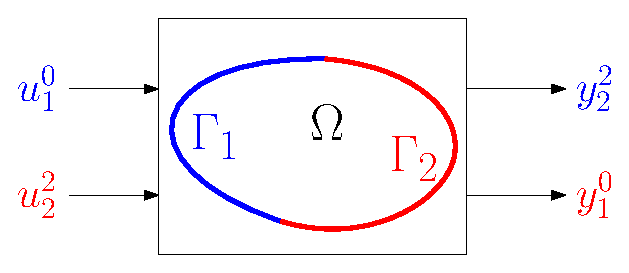
\includegraphics[width=.5\textwidth]{bound_part.eps}
\caption*{Wave equation with mixed \textcolor{blue}{Dirichlet} and \textcolor{red}{Neumann} boundary conditions}
\end{figure}

\end{frame}	

\begin{frame}{The adjoint system}
The initial system
	\begin{equation*}
		\begin{aligned}
			\begin{pmatrix}
				\partial_t p^3 \\
				\partial_t \bm{v}^1\\
			\end{pmatrix} &= 
			-\begin{bmatrix}
				0 & \div \\
				\grad & 0 \\
			\end{bmatrix}
			\begin{pmatrix}
				p^0\\
			 \bm{v}^2\\
			\end{pmatrix}, \\
		\end{aligned}	
	\end{equation*}
The adjoint system

\begin{equation*}
	\begin{aligned}
		\begin{pmatrix}
			\partial_t p^0 \\
			\partial_t \bm{v}^2\\
		\end{pmatrix} &= 
		-\begin{bmatrix}
			0 & \div_w \\
			\grad_w & 0 \\
		\end{bmatrix}
		\begin{pmatrix}
			p^3\\
			\bm{v}^1\\
		\end{pmatrix}, \\
	\end{aligned}	
\end{equation*}

Boundary conditions:
\begin{equation*}
		p^0|_{\Gamma_1} = u^0_1, \qquad
		-\bm{v}^2\cdot \bm{n}|_{\Gamma_2}  = u^{2}_2.
\end{equation*}

\end{frame}

\begin{frame}{Weak formulations}
Introducing Sobolev spaces with boundary conditions	
\begin{equation*}
		H^1_{\Gamma_1}(\Omega) = \{\phi \in H^1(\Omega) |\; \phi|_{\Gamma_1} = 0\}, \qquad
		H^{\div}_{\Gamma_2}(\Omega) = \{\bm{\phi} \in H^{\div}(\Omega) |\; \bm{\phi} \cdot \bm{n}|_{\Gamma_2} = 0\}.
\end{equation*}


\begin{tcolorbox}[nobeforeafter, colframe=theme,title=Primal weak formulation]%%
Find $p^0 \in H^1(\Omega), \; \bm{v}^1 \in H^{\curl}(\Omega)$ such that $p^0|_{\Gamma_1} = u^0_1$ and
\begin{equation*}
	\begin{aligned}
		\inpr[\Omega]{\psi^0}{\partial_t p^0} &= +\inpr[\Omega]{\grad \psi^0}{\bm{v}^1} + \dualpr[\Gamma_2]{\psi^0}{u^2_2}, \\
		\inpr[\Omega]{\bm{\psi}^1}{\partial_t \bm{v}^1} &= -\inpr[\Omega]{\bm{\psi}^1}{\grad {p}^0},
	\end{aligned} \qquad
	\begin{aligned}
		&\forall \psi^0 \in H^1_{\Gamma_1}(\Omega), \\
		&\forall \bm{\psi}^1 \in H^{\curl}(\Omega).
	\end{aligned}
\end{equation*}
\end{tcolorbox} 

\begin{tcolorbox}[nobeforeafter, colframe=theme,title=Dual weak formulation]%%
find $p^3 \in L^2(\Omega), \; \bm{v}^2 \in H^{\div}(\Omega)$ such that $\bm{v}^2 \cdot \bm{n}|_{\Gamma_2} = u^2_2$ and
\begin{equation*}
	\begin{aligned}
		\inpr[\Omega]{\psi^3}{\partial_t p^3} &= -\inpr[\Omega]{\psi_3}{\div\bm{v}^2}, \\
		\inpr[\Omega]{\bm{\psi}^2}{\partial_t \bm{v}^2} &= +\inpr[\Omega]{\div \bm{\psi}^2}{\grad {p}^3} - \dualpr[\Gamma_1]{\bm{\psi}^2 \cdot \bm{n}}{u^0_1},
	\end{aligned} \qquad
	\begin{aligned}
		&\forall \psi^3 \in L^2(\Omega), \\
		&\forall \bm{\psi}^2 \in H^{\div}_{\Gamma_2}(\Omega).
	\end{aligned}
\end{equation*}
\end{tcolorbox} 
The two formulations are uncoupled.
\end{frame}

\begin{frame}{Propagation of an eigensolution in a cavity}
	Box-shaped three-dimensional domain:
	$$\Omega = \{ (x,y,z) \in [0, 1]\times[0, 1/2]\times[0, 1/2] \}.$$ 
	Boundary sub-partitions:
	\begin{equation*}
		\Gamma_1 = \{(x,y,z) \vert \; x=0 \cup y=0 \cup z=0\}, \qquad \Gamma_2 = \{(x, y, z) \vert \; x=1 \cup y=1/2 \cup z=1/2 \}.
	\end{equation*}

Given the functions
\begin{equation*}
	g(x, y, z) = \cos(x) \sin(y) \sin(z), \qquad f(t) = 2 \sin(\sqrt{3} t) + 3 \cos(\sqrt{3} t),
\end{equation*}
an exact solution  is given by
\begin{equation*}\	\begin{aligned}
		p^3_{\mathrm{ex}} &= \star g \diff{f}{t}, \\    
		\bm{v}^1_{\mathrm{ex}} &= -\d{g} f, 
	\end{aligned} \qquad 
	\begin{aligned}
		p^0_{\mathrm{ex}} &= g \diff{f}{t}, \\
		\bm{v}^2_{\mathrm{ex}} &= -\star \d{g} f,
	\end{aligned}
\end{equation*}
The exact solution provides the appropriate inputs to be fed into the system
\begin{equation*}
	u^0_1 =p^0_{\mathrm{ex}}|_{\Gamma_1}, \qquad u^2_2 =  -\bm{v}^2_{\mathrm{ex}} \cdot \bm{n}\vert_{\Gamma_2}.
	\end{equation*}
\end{frame}


\begin{frame}{Results obtained with a direct solver and implicit midpoint}
	
	\only<1>{
		
		\begin{columns}		
			\begin{column}{.45\textwidth}
				\includemedia[
				addresource=/home/andrea/Videos/CandidatureISAE/Wavep33D.mp4,
				activate=pageopen, 
				deactivate=onclick,
				width=7cm, height=6cm,
				flashvars={
					source=/home/andrea/Videos/CandidatureISAE/Wavep33D.mp4
					&%
					autoPlay=true&%
					loop=true%
				}
				]{}{VPlayer.swf}
				$p^3$
			\end{column}
			\begin{column}{.45\textwidth}
				\includemedia[
				addresource=/home/andrea/Videos/CandidatureISAE/Wavep03D.mp4,
				activate=pageopen, 
				deactivate=onclick,
				width=7cm, height=6cm,
				flashvars={
					source=/home/andrea/Videos/CandidatureISAE/Wavep03D.mp4&%
					autoPlay=true&%
					loop=true%
				}
				]{}{VPlayer.swf}
				$p^0$
			\end{column}
		\end{columns}	
	}
	
	\only<2>{
		
		\begin{columns}		
			\begin{column}{.45\textwidth}
				\includemedia[
				addresource=/home/andrea/Videos/CandidatureISAE/Waveu23D.mp4,
				activate=pageopen, 
				deactivate=onclick,
				width=7cm, height=6cm,
				flashvars={
					source=/home/andrea/Videos/CandidatureISAE/Waveu23D.mp4
					&%
					autoPlay=true&%
					loop=true%
				}
				]{}{VPlayer.swf}
				$\bm{v}^2$
			\end{column}
			\begin{column}{.45\textwidth}
				\includemedia[
				addresource=/home/andrea/Videos/CandidatureISAE/Waveu13D.mp4,
				activate=pageopen, 
				deactivate=onclick,
				width=7cm, height=6cm,
				flashvars={
					source=/home/andrea/Videos/CandidatureISAE/Waveu13D.mp4&%
					autoPlay=true&%
					loop=true%
				}
				]{}{VPlayer.swf}
				$\bm{v}^1$
			\end{column}
			
		\end{columns}	
	}
	
	\only<3>{	
		\begin{figure}
			\centering
			\subfloat[][$||p^3_h - {p}_{\text{ex}}||_{L^2}$]{%
				\label{fig:err_p3}%
				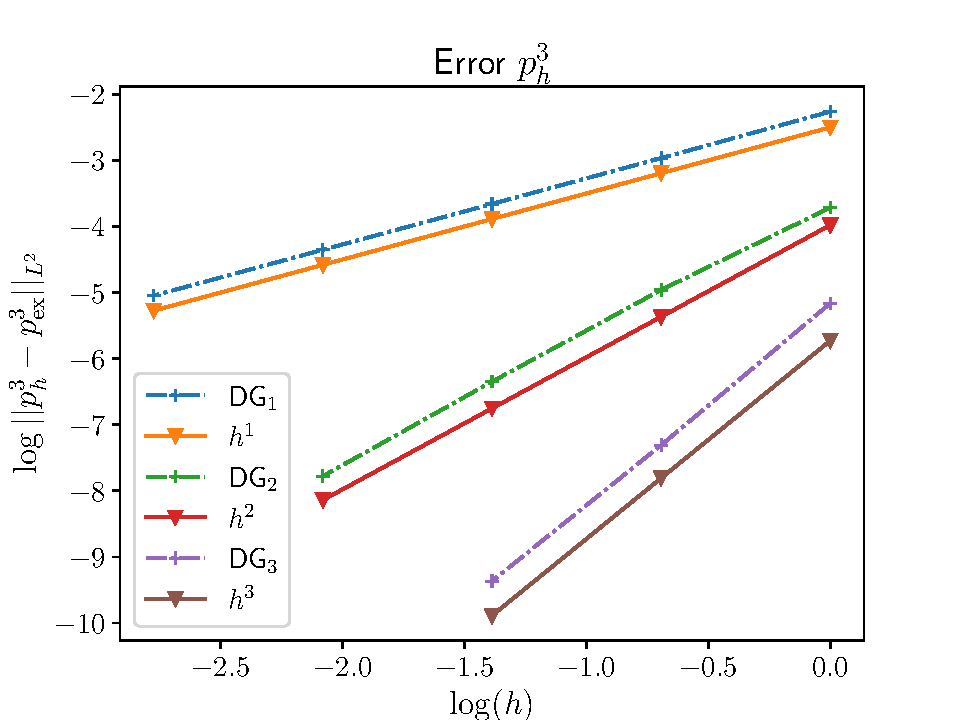
\includegraphics[width=0.48\columnwidth]{p_3_3D_DN.pdf}}%
			\hspace{8pt}%
			\subfloat[][$||p^0_h - {p}_{\text{ex}}||_{L^2}$]{%
				\label{fig:err_p0}%
				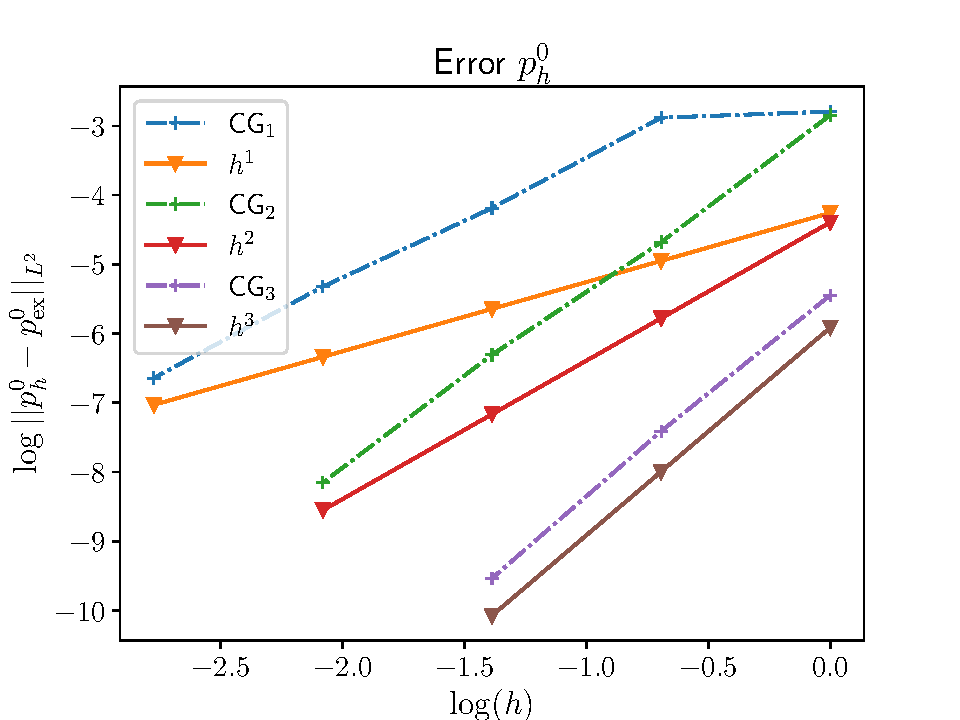
\includegraphics[width=0.48\columnwidth]{p_0_3D_DN.pdf}}%
			\caption*{Convergence rate for $p$}%
		\end{figure}
	}
	\only<4>{	
		\begin{figure}
			\centering
			\subfloat[][$||\bm{v}^1_h - \bm{v}_{\text{ex}}||_{L^2}$]{%
				\label{fig:err_u1}%
				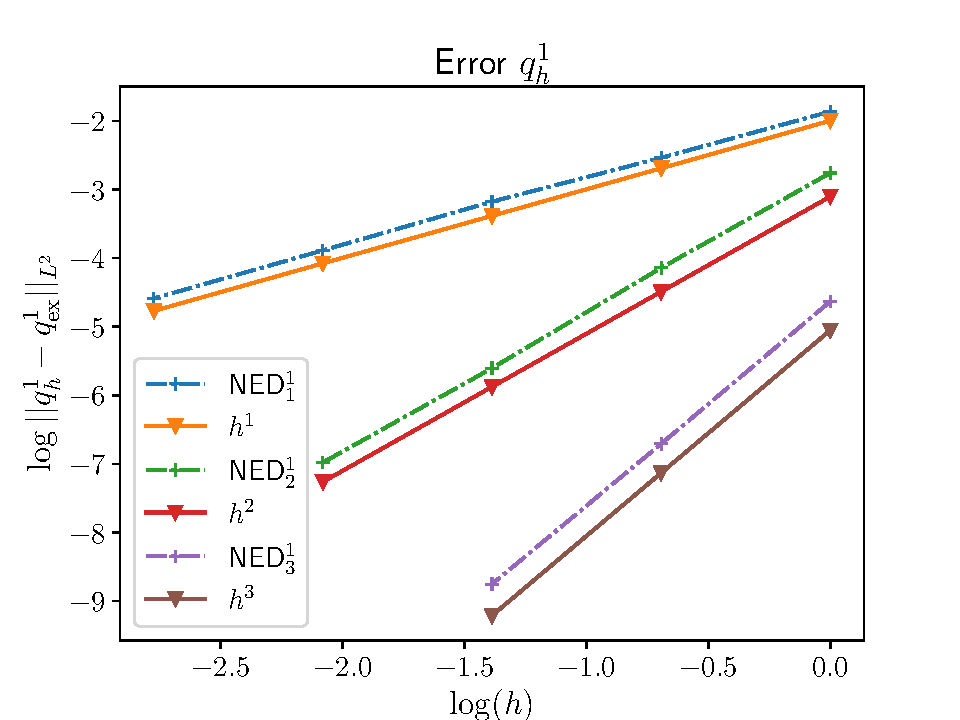
\includegraphics[width=0.48\columnwidth]{q_1_3D_DN.pdf}}
			\hspace{8pt}%
			\subfloat[][$||\bm{v}^2_h - \bm{v}_{\text{ex}}||_{L^2}$]{%
				\label{fig:err_u2}%
				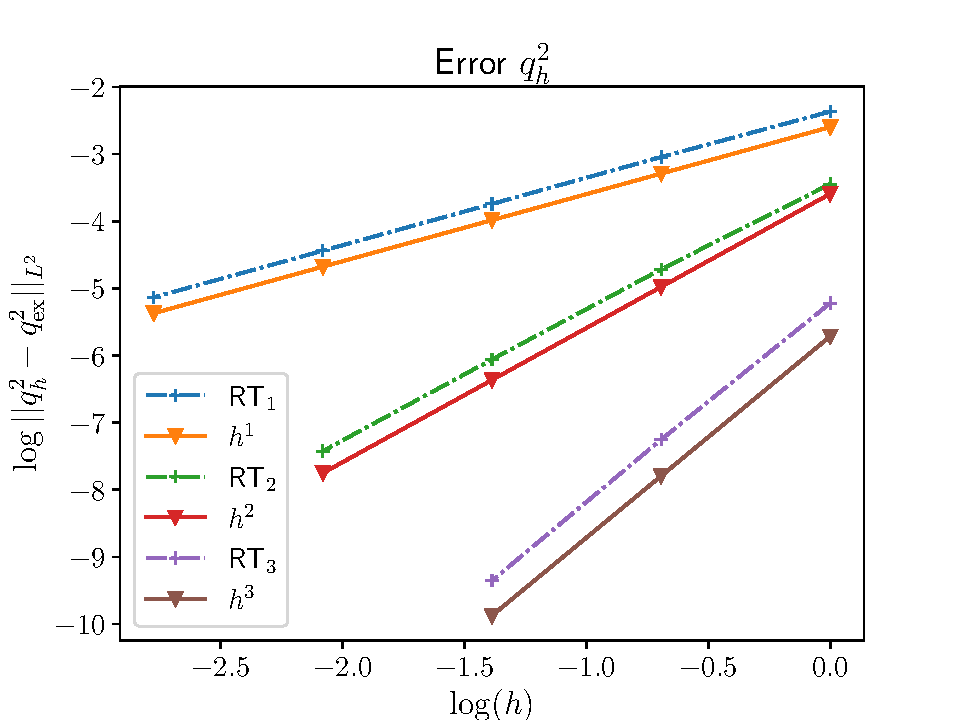
\includegraphics[width=0.48\columnwidth]{q_2_3D_DN.pdf}}
			\caption*{Convergence rate for $\bm{v}$}%
		\end{figure}
	}
	\only<5>{
		\begin{figure}
			\centering
			\subfloat[][$||p^3_h - p^0_h||_{L^2}$]{%
				\label{fig:diff_p30}%
				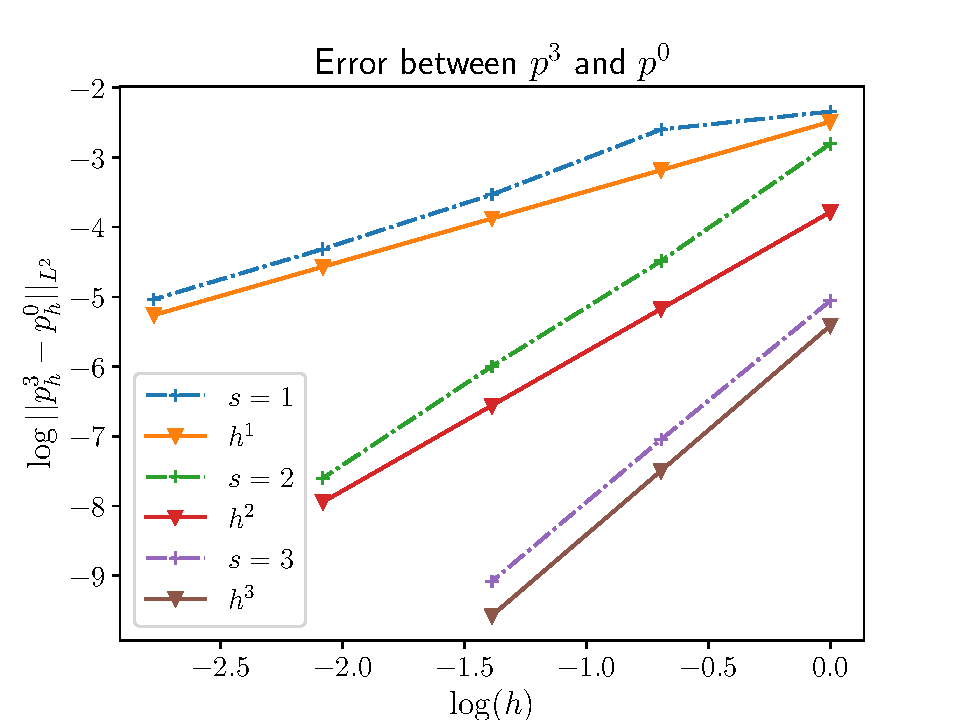
\includegraphics[width=0.48\columnwidth]{p_30_3D_DN.pdf}}%
			\hspace{8pt}%
			\subfloat[][$||\bm{v}^1_h - \bm{v}^2_h||_{L^2}$]{%
				\label{fig:diff_q12}%
				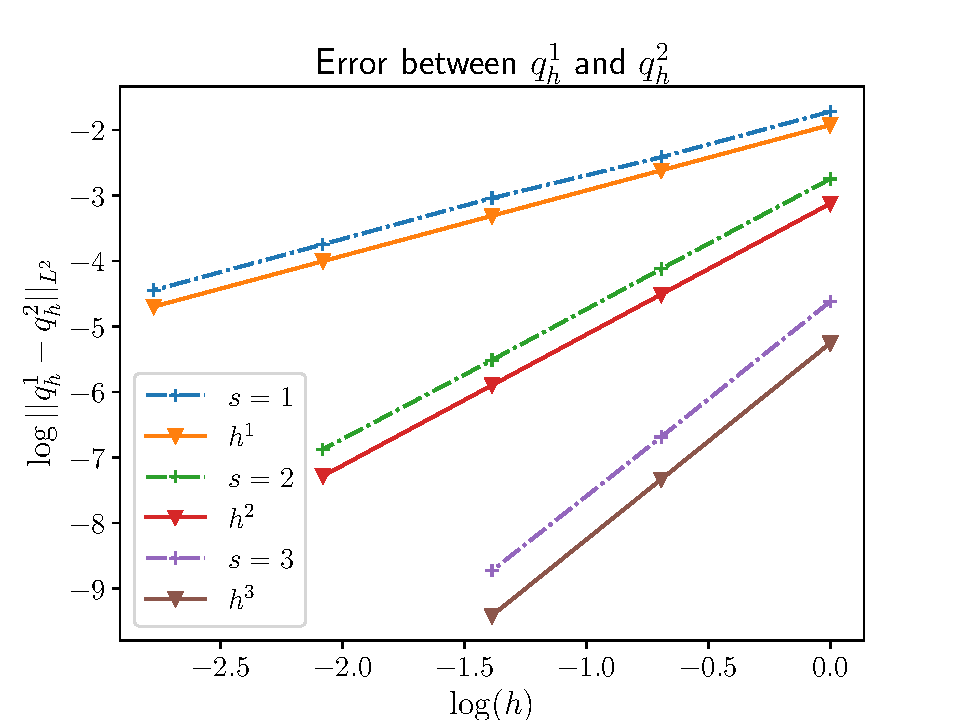
\includegraphics[width=0.48\columnwidth]{q_12_3D_DN.pdf}}%
			\caption*{$L^2$ norm of the difference between dual representation.}%
		\end{figure}
	}
	
	
	
\end{frame}

\begin{frame}{Conclusion}
	The open character of pH systems has the \textbf{potential to improve the status quo} of multiphysics simulation in industry.  \\
	\vspace{.3cm}
	\begin{tcolorbox}[nobeforeafter, colframe=theme,title=First pH systems need to become an established physical theory]%%
	\begin{itemize}
		\item unique definition of (infinite dimensional) pH system on manifolds;
		\item incorporation of geometric and functional analytic aspects;
		\item extension of the geometric theory to continuum mechanics;
	\end{itemize}
	\end{tcolorbox} 
	\vspace{.3cm}\\
	\begin{tcolorbox}[nobeforeafter, colframe=theme,title=For engineering pH systems need to be more efficient than the available tools]%%
	\begin{itemize}
		\item efficient strategy for the resolution of large-scale pH models;
		\item model reduction of models arising from PDEs discretization;
		\item more open-source code and benchmark problems.
	\end{itemize}
	\end{tcolorbox}

\end{frame}
	
\begin{frame}[allowframebreaks]{Bibliography}
	%\bibliographystyle{unsrt}
	%\nocite{*}
	\printbibliography
\end{frame}

	\appendix
	
	
	
	
\end{document}